%
% $RCSfile: hierarchical_model.tex,v $
%
% Copyright (C) 2002-2008. Christian Heller.
%
% Permission is granted to copy, distribute and/or modify this document
% under the terms of the GNU Free Documentation License, Version 1.1 or
% any later version published by the Free Software Foundation; with no
% Invariant Sections, with no Front-Cover Texts and with no Back-Cover
% Texts. A copy of the license is included in the section entitled
% "GNU Free Documentation License".
%
% http://www.cybop.net
% - Cybernetics Oriented Programming -
%
% http://www.resmedicinae.org
% - Information in Medicine -
%
% Version: $Revision: 1.1 $ $Date: 2008-08-19 20:41:07 $ $Author: christian $
% Authors: Christian Heller <christian.heller@tuxtax.de>
%

\subsubsection{Hierarchical Model}
\label{hierarchical_model_heading}
\index{Hierarchical Model Approach}
\index{Composition}
\index{Directed Acyclical Graph}
\index{DAG}
\index{Composite Pattern}

The \emph{Hierarchical Model} as yet more generalised form of data representation
is based on \emph{Composition} as one of the principles of human thinking
(section \ref{abstraction_heading}). Its tree structure -- ideally in form of a
\emph{Directed Acyclical Graph} (DAG) (section \ref{terminology_heading}) --
allows dynamic extensions of data types, by simply adding child nodes (parts)
to a parent node (whole), in the knowledge tree.

\begin{figure}[ht]
    \begin{center}
        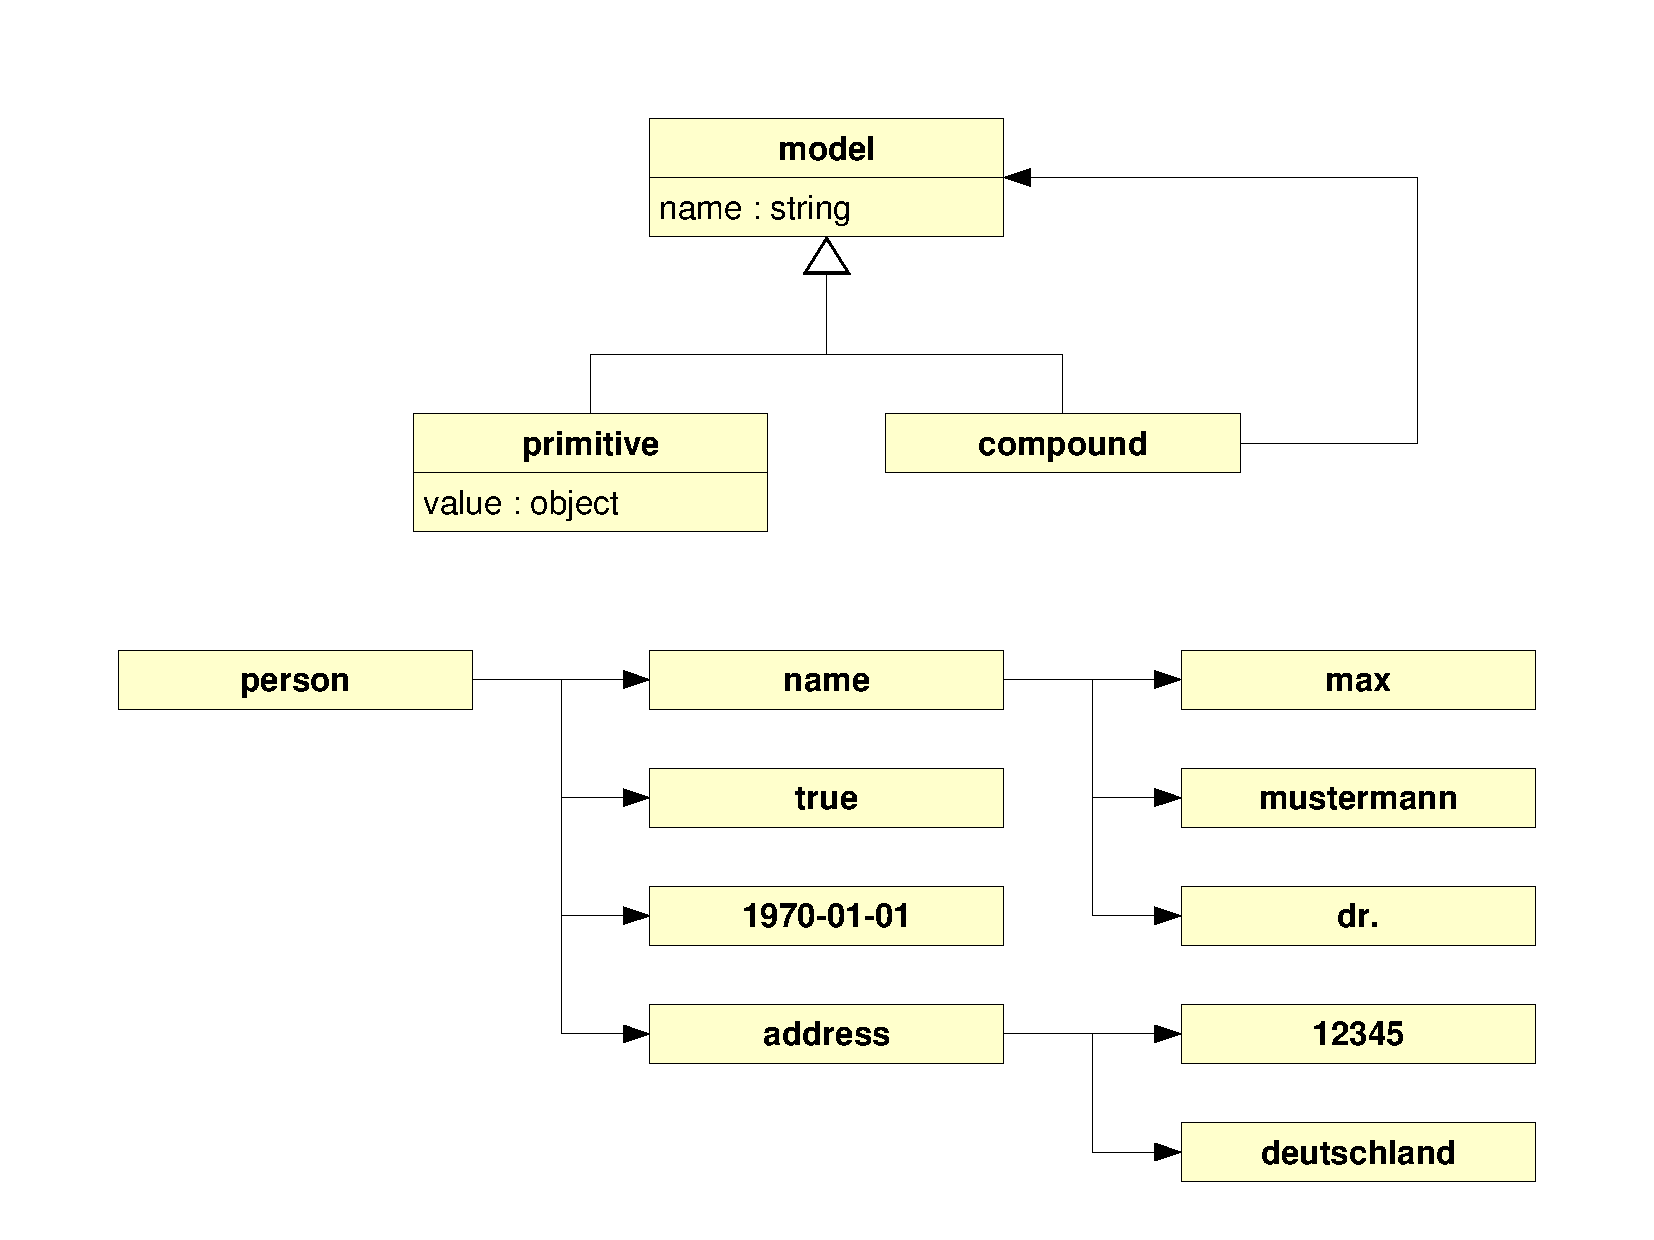
\includegraphics[scale=0.3,angle=-90]{graphic/hierarchical.pdf}
        \caption{Hierarchical Model Approach (adapted from \cite{archetypes})}
        \label{hierarchical_figure}
    \end{center}
\end{figure}

The upper half of figure \ref{hierarchical_figure} shows the \emph{Composite}
software pattern (section \ref{composite_heading}). Its classes do not contain
hard-coded attributes; two exceptions are the \emph{Primitive} class' attribute
\emph{value} and the \emph{Compound} class' dynamically extensible structure.
The structure may be a list, and it stores all of the compound's parts in it.
Parts may be primitiva or compounds themselves. As already proposed by the
\emph{Semi Structured Model} before, each part is identified by a name that is
unique within its compound. The diagram in the lower half of the figure clearly
shows the hierarchical tree structure of runtime instances.

The only open issue when using purely hierarchical models is that the semantics
-- the actual domain concepts -- is lost. Knowledge models, together with their
parts and meta information about these (position, size, colour, constraints --
as described in section \ref{human_thinking_heading}), thus need to be defined
somewhere else. The later section \ref{knowledge_representation_heading}
proposes a generic knowledge schema for doing this.
